\documentclass[english]{beamer}
%Gummi|065|=)
\usepackage{xeCJK}
%\usepackage{times}
\usepackage[T1]{fontenc}
\setCJKmainfont[BoldFont=SimHei]{SimSun}
\setCJKmonofont{SimSun}% 设置缺省中文字体
%\parindent 2em 
\usepackage{graphics}
\usetheme{Antibes}
\title{\textbf{A Brief Introduction to the Working Principles of The Light Emiting Diode}}
\author[Teren]{Teren Liu\\ Ziyou Wang, Chaoyue Liu, Xinyan Zhang, Shitong Chen, Bao Wang, Ziyu Yin, Cheng Ran,                Pu Feng\\{teren.liu@hit.edu.cn}}
\date{2015-11-12}
\begin{document}

\maketitle

\begin{frame}
	\frametitle{An Brief Introduction to the LED}
	A light-emitting diode (LED) is a two-lead semiconductor light source. It is a p–n junction diode, which emits light when activated. When a suitable voltage is applied to the leads, electrons are able to recombine with electron holes within the device, releasing energy in the form of photons. This effect is called electroluminescence, and the color of the light (corresponding to the energy of the photon) is determined by the energy band gap of the semiconductor.
\end{frame}
\begin{frame}{Energy structure in LED}
	\includegraphics[height=0.6\textwidth]{f1.png}
\end{frame}
\begin{frame}{Working Principle of the Light Emitting }
	A P-N junction can convert the absorbed light energy into its proportional electric current. The same process is reversed here (i.e. the P-N junction emits light when electrical energy is applied on it). This phenomenon is generally called electroluminescence, which can be defined as the emission of light from a semi-conductor under the influence of an electric field. The charge carriers recombine in a forward P-N junction as the electrons cross from the N-region and recombine with the holes existing in the P-region. Free electrons are in the conduction band of energy levels, while holes are in the valence energy band. Thus the energy level of the holes will be lesser than the energy levels of the electrons. Some part of the energy must be dissipated in order to recombine the electrons and the holes. This energy is emitted in the form of heat and light.
\end{frame}
\begin{frame}{Working Principle of the Light Emitting}
	But:
	
	The electrons dissipate energy in the form of heat for silicon and germanium diodes but in gallium arsenide phosphide (GaAsP) and gallium phosphide (GaP) semiconductors, the electrons dissipate energy by emitting photons.
\end{frame}
\begin{frame}{Reason}
	The different Energy Gap Structure Makes the different emitting type.
	
	Silicon and germanium is the INDIRECT BAND GAP crystal, while the GaAsP/... is the DIRECT BAND GAP crystal.
\end{frame}
\begin{frame}{Direct/Indirect Band Gap}
	\includegraphics[width=0.5\textwidth]{f3.png}
	\includegraphics[width=0.5\textwidth]{f2.png}
\end{frame}
\begin{frame}{Heterojunction}
	In order to increase the quantum dropping efficiency, Modern LED use the heterojuntion structure. more information of the Heterojunction is in our further semiconductor course.
	
	\includegraphics[width=0.7\textwidth]{f5}
\end{frame}
\begin{frame}{White LED}
	Here are the current ways to achieve the goal of White light "emitting".
	\begin{itemize}
		\item blue LED + green LED + red LED (color mixing; can be used as backlighting for displays)
		\item near-UV or UV LED + RGB phosphor (an LED producing light with a wavelength shorter than blue's is used to excite an RGB phosphor)
		\item blue LED + yellow phosphor (two complementary colors combine to form white light; more efficient than first two methods and more commonly used)
	\end{itemize}
\end{frame}
\begin{frame}{OLED}
	\includegraphics[width=0.5\textwidth]{homo}
	\includegraphics[width=0.5\textwidth]{oled}
	
	1. Cathode (−), 2. Emissive Layer, 3. Emission of radiation, 4. Conductive Layer, 5. Anode (+)
\end{frame}
\begin{frame}{Quantum Dot LED}
	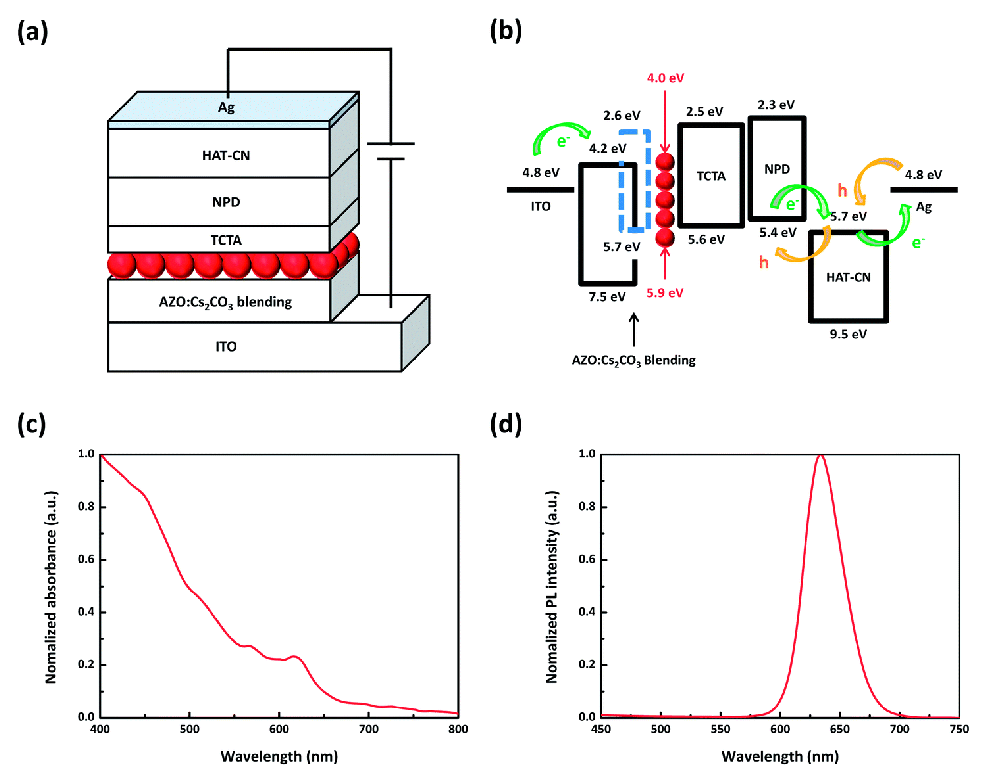
\includegraphics[width=0.6\textwidth]{qlede}
	%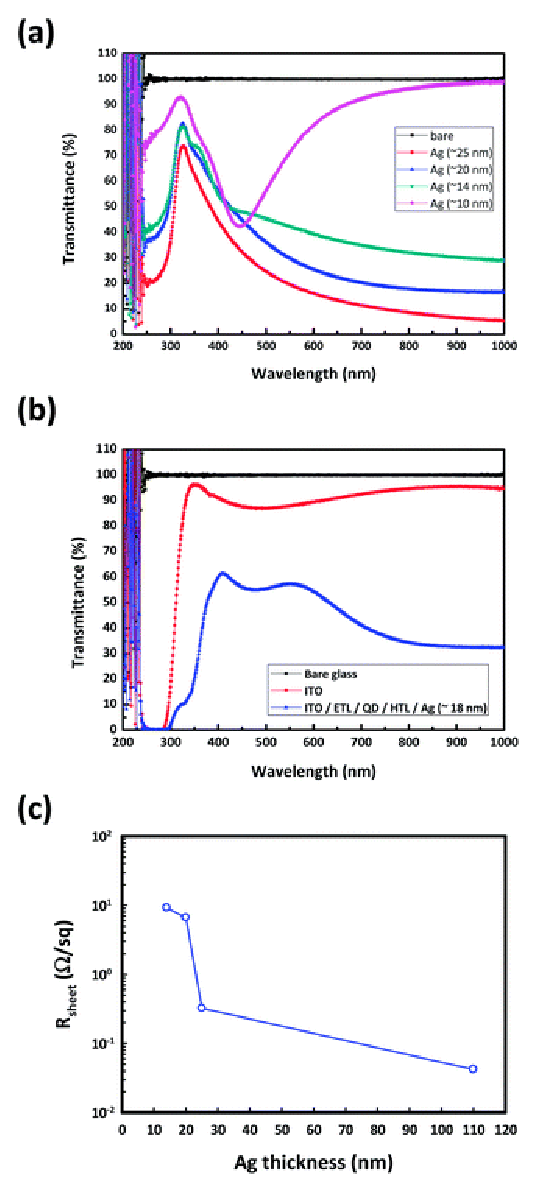
\includegraphics[width=0.2\textwidth]{qled1e}
	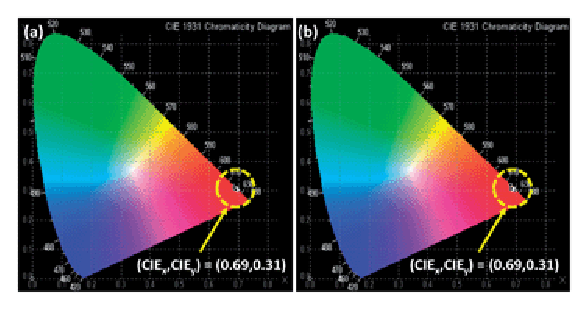
\includegraphics[width=0.5\textwidth]{qled2e}
\end{frame}
\end{document}
